\documentclass[10pt]{beamer}
\usetheme[
%%% option passed to the outer theme
%    progressstyle=fixedCircCnt,   % fixedCircCnt, movingCircCnt (moving is deault)
  ]{Feather}
  
% If you want to change the colors of the various elements in the theme, edit and uncomment the following lines

% Change the bar colors:
\setbeamercolor{Feather}{fg=red!80!black,bg=red!60!black}
\setbeamercolor{block title}{bg=red!80!black, fg=white}
\setbeamercolor{block body}{bg=white, fg=black}

% Change the color of the structural elements:
\setbeamercolor{structure}{fg=black}

% Change the frame title text color:
\setbeamercolor{frametitle}{fg=yellow}

% Change the normal text color background:
%\setbeamercolor{normal text}{fg=black,bg=gray!10}

%-------------------------------------------------------
% INCLUDE PACKAGES
%-------------------------------------------------------
\usepackage{ifpdf}
\usepackage{xcolor}
\usepackage{graphicx} 
\usepackage{caption}
\usepackage{subcaption}
\usepackage{multicol}
\usepackage{animate}
\ifpdf
\DeclareGraphicsRule{*}{mps}{*}{}
\else
% Recent LaTeX versions donât require the next line
% \DeclareGraphicsRule{*}{eps}{*}{}
\fi

\usepackage[english, french]{babel}
\usepackage[utf8]{inputenc}
%\usepackage[TS1,T1]{fontenc}
%\usepackage{helvet}
\usepackage{fourier}
%\usepackage{hyperref}
%\usepackage{lmodern}
%\usepackage{mathrsfs}
\usepackage{natbib}
\usepackage{amsmath,amssymb,amsfonts,graphicx,shorttoc,textpos,caption,here, yfonts}
\usepackage{verbatim,enumerate,dsfont,fancyhdr,setspace,array}

%\usepackage[style=authoryear]{biblatex}
%\renewcommand*{\nameyeardelim}{\addcomma\addspace}


\graphicspath{{Feathergraphics/}}
%\bibliography{biblio1}
%\DeclareCiteCommand{\cite}
%{\usebibmacro{prenote}}
%{\usebibmacro{citeindex}%
%\usebibmacro{cite}}
%{\multicitedelim}
%{\usebibmacro{cite:postnote}}
%\usefonttheme[onlymath]{serif}
%\newbibmacro*{cite}{%
%\usebibmacro{cite:citepages}%
%\ifciteseen
%	{\iffieldundef{shorthand}
%		{\usebibmacro{cite:short}}
%		{\usebibmacro{cite:shorthand}}}
%	{\usebibmacro{cite:full}}}
%
%\renewbibmacro*{cite}{%
%\usebibmacro{cite:citepages}%
%{\usebibmacro{cite:full}}}
%-------------------------------------------------------
% DEFFINING AND REDEFINING COMMANDS
%-------------------------------------------------------

% colored hyperlinks
\newcommand{\chref}[2]{
  \href{#1}{{\usebeamercolor[bg]{Feather}#2}}
}
\DeclareMathOperator*{\argmin}{arg\,min}
%\bibliographystyle{apalike}
%\renewcommand\bibfont{\scriptsize}
\DeclareMathOperator*{\Argmin}{Arg\,min}
\setbeamertemplate{frametitle continuation}[from second]

%-------------------------------------------------------
% INFORMATION IN THE TITLE PAGE
%-------------------------------------------------------

\title[Bayesian minimax and oracle optimality in an inverse Gaussian sequence space model] % [] is optional - is placed on the bottom of the sidebar on every slide
{ % is placed on the title page
     \textbf{Bayesian minimax and oracle optimality in an inverse Gaussian sequence space model}
}


\subtitle[loizeau@math.uni-heidelberg.de] % [] is optional - is placed on the bottom of the sidebar on every slide
{ % is placed on the title page
    % \textit{loizeau@math.uni-heidelberg.de}
}


\institute[Ruprecht-Karls-Universität Heidelberg]
{
  
  \begin{flushright}Ruprecht-Karls-Universität Heidelberg\end{flushright}
  %there must be an empty line above this line - otherwise some unwanted space is added between the university and the country (I do not know why;( )
}

\date{\begin{flushleft}In collaboration with Jan Johannes\end{flushleft}}

\author[Xavier Loizeau] % [] is optional - is placed on the bottom of the sidebar on every slide
{ % is placed on the title page
      \textit{Xavier Loizeau\\      $9^{th}$ of March 2016}
}
%-------------------------------------------------------
% THE BODY OF THE PRESENTATION
%-------------------------------------------------------

\begin{document}
%-------------------------------------------------------
% THE TITLEPAGE
%-------------------------------------------------------

{\1% % this is the name of the PDF file for the background
\begin{frame}[plain,noframenumbering] % the plain option removes the header from the title page, noframenumbering removes the numbering of this frame only
  \titlepage % call the title page information from above
\end{frame}}

\AtBeginSection[]{
\begin{frame}[noframenumbering]{Contents}
\setcounter{tocdepth}{1}
%\begin{multicols}{2}
\tableofcontents[sectionstyle=show/shaded, subsectionstyle=show/show/hide]
%\end{multicols}
\end{frame}
}

%\begin{frame}{Contents}
%\setcounter{tocdepth}{1}
%\tableofcontents
%\end{frame}

%-------------------------------------------------------
\section{Introduction}
%-------------------------------------------------------
\subsection{Considered model}

\begin{frame}{Considered model}{Indirect sequence space model}

Consider an indirect Gaussian sequence space model consisting of:
\begin{itemize}
\item<2-> an unknown parameter of interest $\left(\theta^{\circ}_{j}\right)_{j \in \mathbb{N}} = \theta^{\circ}$;
\item<3-> a polynomially decreasing multiplicative sequence $\left(\lambda_{j}\right)_{j \in \mathbb{N}} = \lambda$ converging to $0$;
\item<4-> observations $\left(Y_{j}\right)_{j \in \mathbb{N}} = Y$, contaminated by an additive independent centered Gaussian noise with variance $n^{-1}$;
\end{itemize}

\bigskip

\textcolor{red!90!black}{\[Y = \left(\theta^{\circ}_{j} \cdot \lambda_{j} + \sqrt{n}^{-1} \cdot \xi_{j}\right)_{j \in \mathbb{N}}, \quad \left(\xi_{j}\right)_{j \in \mathbb{N}} \sim_{iid} \mathcal{N}\left(0, 1\right).\]}

The goal is to recover $\theta^{\circ}$ and prove asymptotic optimality.
\end{frame}


\begin{frame}{Considered model}{Illustration}
\begin{columns}[c]
	\begin{column}{3cm}
		\begin{alignat*}{2}
&\color{green!90!black} \sum\limits_{j \geq 1}\theta^{\circ}_{j} \lambda_{j}^{t} \cdot \psi_{j}(x);&&\\
&\color{red!90!black} \sum\limits_{j \geq 1} Y_{j} \cdot \psi_{j}(x);&&\\
&\lambda_{j}^{t} = \exp\left[-\left(j + 1\right)^{2} \cdot t \right]&&\\
&\lambda_{j}^{t} = \exp\left[-2 \cdot \log\left(j + 1\right) \cdot t \right]&&
		\end{alignat*}
	\end{column}
	\begin{column}{8cm}
		\begin{center}
			\animategraphics[loop,controls,width=40ex]{10}{animation/test-}{0}{147}
		\end{center}
	\end{column}
\end{columns}
\end{frame}

%\begin{frame}{Considered model}{Background}
%A motivation for the model is the \textcolor{red!90!black}{Backwards heat equation}.
%
%See for example \textbf{\citet{HEMHAN}}.
%
%\medskip
%
%Also this model belongs to the wide family of the \textbf{inverse Sequence Space models}, meaning that a method for one of the models has chances to find an echo in another (for example deconvolution model, non parametric regression etc).
%\end{frame}

\subsection{A popular frequentist method}
\begin{frame}{A popular frequentist method}{Projection estimators}
From a frequentist point of view, a natural method to answer this problem is:

\bigskip

\begin{itemize}
\setlength\itemsep{2em}
\item<1-> for any $j$ in $\mathbb{N}$, consider an unbiased estimator $\textcolor{red!90!black}{\widetilde{\theta}_{j} = \frac{Y_{j}}{\lambda_{j}}} = \theta^{\circ} + \frac{1}{\sqrt{n}\cdot\lambda_{j}} \xi_{j};$
\item<2-> family of projection estimators $\left\{\left(\widetilde{\theta}^{m}_{j}\right)_{j \in \mathbb{N}} : \forall j \in \mathbb{N}, \quad \widetilde{\theta}^{m}_{j} = \widetilde{\theta}_{j} \mathds{1}_{\left\{j \leq m\right\}} \right\};$
\item<3-> define a method to select $m$ in a satisfactory way.
\end{itemize}
\end{frame}

\begin{frame}{A popular frequentist method}{Model selection}
To do so, use model selection by penalized contrast:

\medskip

\begin{itemize}
\setlength\itemsep{1em}
\item<1-> select $\textcolor{red!90!black}{\widehat{m} := \argmin\limits_{m \in \llbracket 1, n\rrbracket}\left\{pen(m) + \gamma(m)\right\}};$
\item<2-> for any $m$ in $\llbracket 1, n\rrbracket$ define $pen(m) := 3 \cdot m;$
\item<3-> for any $m$ in $\llbracket 1, n\rrbracket$ define $\gamma(m) := -\sum\limits_{j = 1}^{m} Y_{j}^{2}.$
\end{itemize}

\medskip

Thus an estimator is defined by : $\textcolor{red!90!black}{\widehat{\theta} = \left(\widetilde{\theta}^{\widehat{m}}_{j}\right)_{j \in \mathbb{N}}}.$

\medskip

\textbf{\citet{PM}} gives an overview of this method.
\end{frame}

\subsection{Illustration}
\begin{frame}{Illustration}{Direct case}
\begin{figure}
\centering
 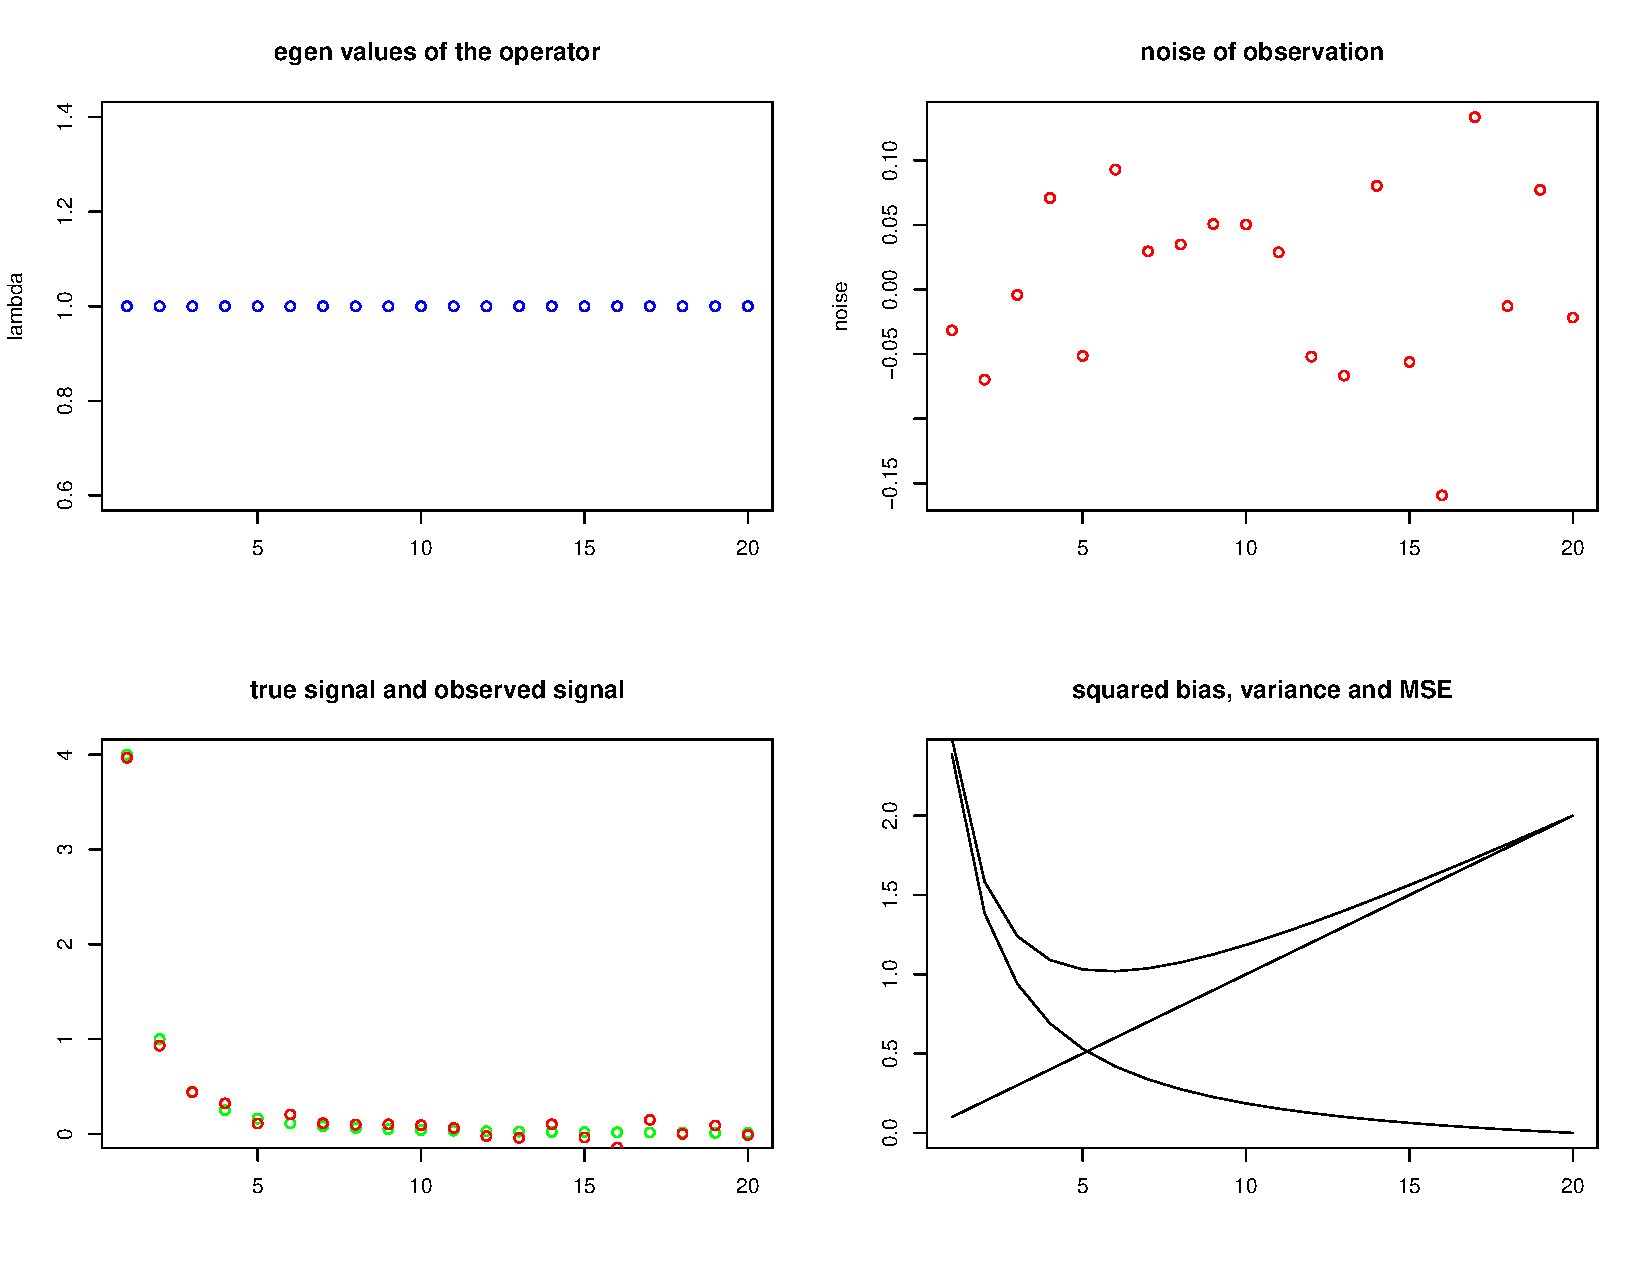
\includegraphics[width=.8\linewidth]{direct-case.pdf}
\caption{MSE of projection estimators in the direct case}\label{DC}
\end{figure}
\end{frame}

\begin{frame}{Illustration}{Inverse case}
\begin{figure}
\centering
 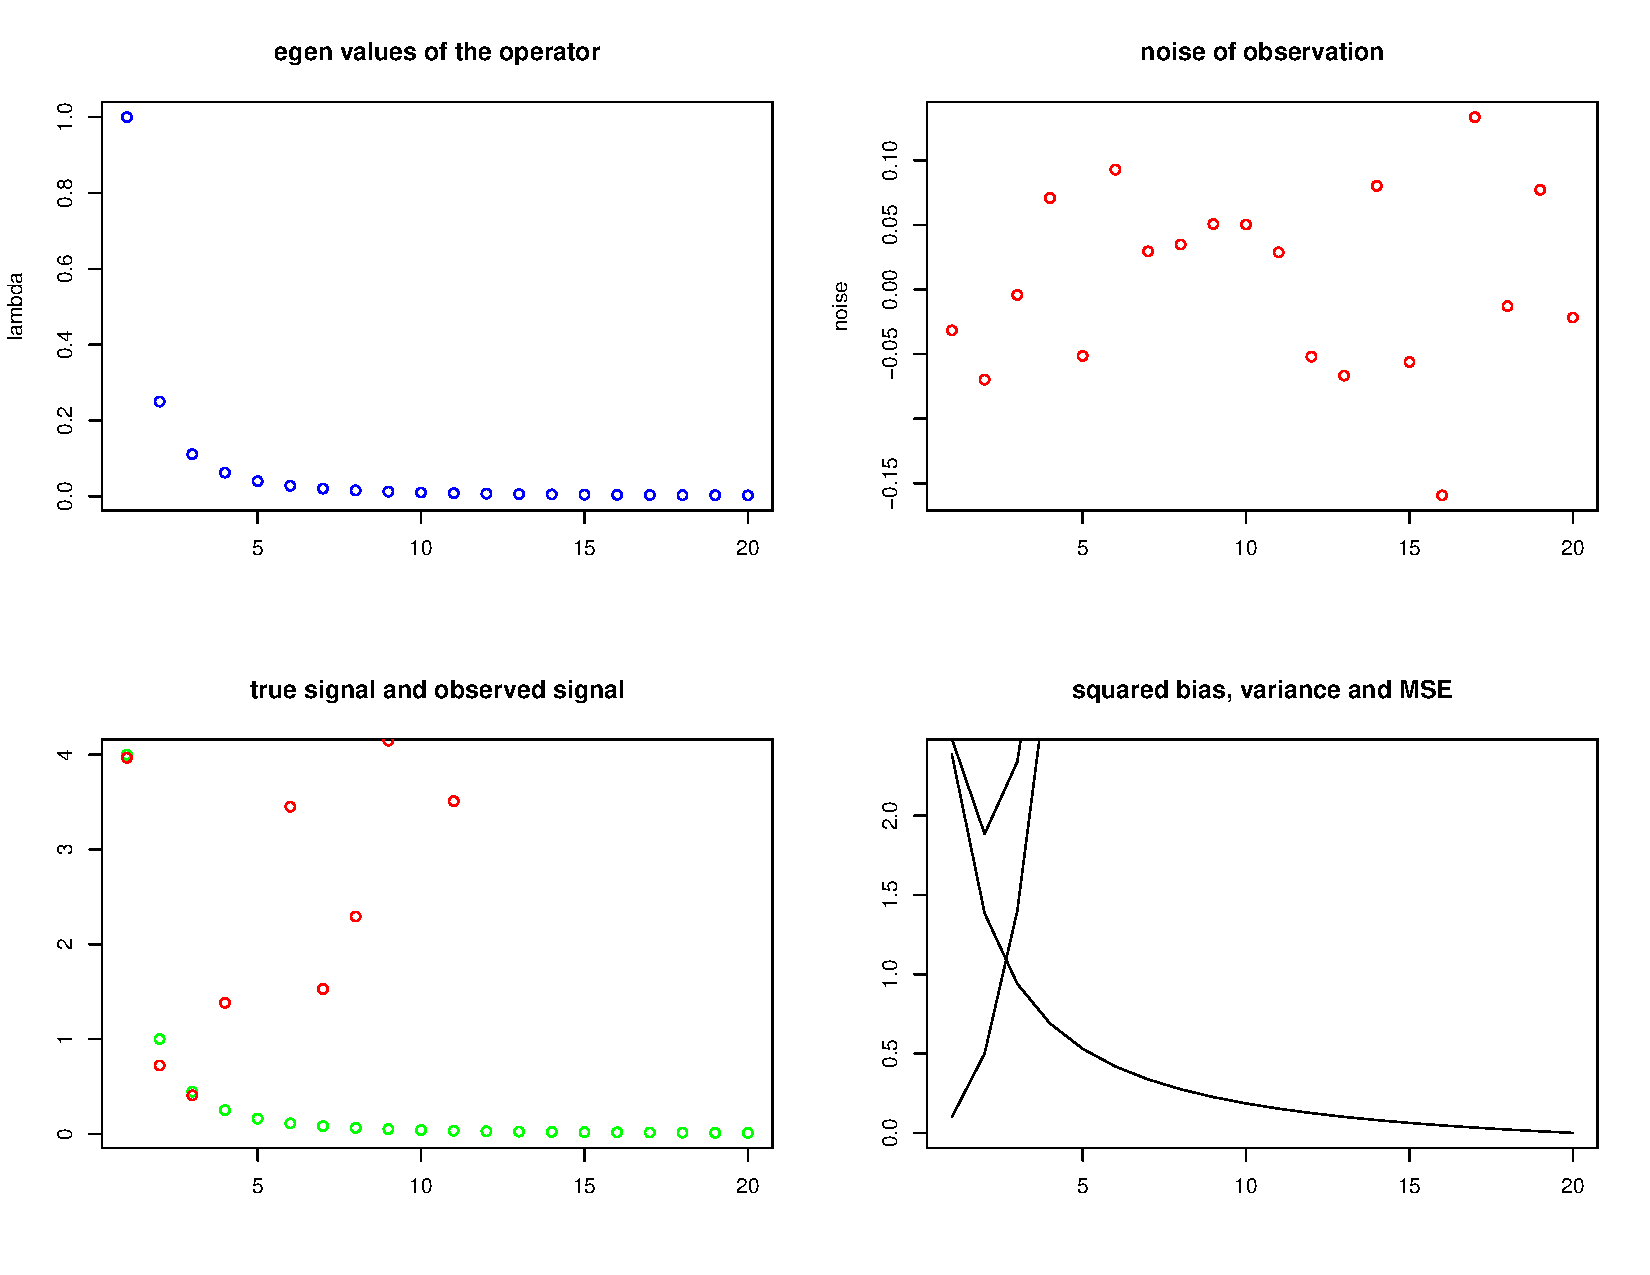
\includegraphics[width=.8\linewidth]{mildly-illposed.pdf}
\caption{MSE of projection estimators in the mildly ill-posed case}\label{MIP}
\end{figure}
\end{frame}

\subsection{Bayesian point of view}
\begin{frame}{Bayesian point of view}{Bayesian fondamental paradigm}
The problem is here treated from a Bayesian point of view:

\bigskip

\begin{itemize}
\setlength\itemsep{3em}
\item<1-> the parameter $\boldsymbol{\theta}$ is a random variable with \textcolor{red!90!black}{prior} $\textcolor{red!90!black}{\mathbb{P}_{\boldsymbol{\theta}}};$
\item<2-> given $\boldsymbol{\theta},$ the \textcolor{red!90!black}{likelihood} of $Y$ is $\textcolor{red!90!black}{\mathbb{P}_{Y \vert \boldsymbol{\theta}}^{n}} = \mathcal{N}\left(\boldsymbol{\theta} \cdot \lambda, n^{-1} \mathcal{I}\right);$
\item<3-> we are interested in the \textcolor{red!90!black}{posterior distribution} $\textcolor{red!90!black}{\mathbb{P}_{\boldsymbol{\theta} \vert Y}^{n}} \propto \mathbb{P}_{Y \vert \boldsymbol{\theta}}^{n} \cdot \mathbb{P}_{\boldsymbol{\theta}}.$
\end{itemize}
\end{frame}

\begin{frame}{Bayesian point of view}{Iterated posterior distribution}
In the spirit of \textbf{\citet{OBJJ}}, we then generate a posterior family by introducing an \textcolor{red!90!black}{iteration parameter $\eta$}:
\begin{itemize}
\setlength\itemsep{1em}
\item<1-> for $\textcolor{red!90!black}{\eta = 1}$, the prior distribution is $\mathbb{P}_{\boldsymbol{\theta}^{1}} = \mathbb{P}_{\boldsymbol{\theta}},$ the likelihood $\mathbb{P}_{Y^{1} \vert \boldsymbol{\theta}^{1}}^{n} = \mathbb{P}_{Y \vert \boldsymbol{\theta}}^{n}$ and the posterior distribution is $\mathbb{P}_{\boldsymbol{\theta}^{1} \vert Y^{1}}^{n} = \mathbb{P}_{\boldsymbol{\theta}\vert Y}^{n};$
\item<2-> for $\textcolor{red!90!black}{\eta = 2},$ we take the posterior for $\eta = 1$ as prior, hence, the \textcolor{red!90!black}{prior is} $\textcolor{red!90!black}{\mathbb{P}_{\boldsymbol{\theta}^{2}}^{n} = \mathbb{P}_{\boldsymbol{\theta}^{1} \vert Y^{1}}^{n}},$ the likelihood does not change $\mathbb{P}_{Y^{2} \vert \boldsymbol{\theta}^{2}}^{n} = \mathbb{P}_{Y \vert \boldsymbol{\theta}}^{n}$ and we compute the posterior with the same observations $Y$, which we note $\mathbb{P}_{\boldsymbol{\theta}^{2} \vert Y^{2}}^{n};$
\item<3-> ...
\item<4-> for any value of $\textcolor{red!90!black}{\eta > 1},$ the prior is $\textcolor{red!90!black}{\mathbb{P}_{\boldsymbol{\theta}^{\eta}}^{n} = \mathbb{P}_{\boldsymbol{\theta}^{\eta-1} \vert Y^{\eta - 1}}}$ and we compute the posterior with the same likelihood $\textcolor{red!90!black}{\mathbb{P}_{Y^{\eta} \vert \boldsymbol{\theta}^{\eta}}^{n} = \mathbb{P}_{Y \vert \boldsymbol{\theta}}^{n}}$ and same observations $Y$ which gives $\textcolor{red!90!black}{\mathbb{P}_{\boldsymbol{\theta}^{\eta} \vert Y^{\eta}}^{n}}.$
\end{itemize}
\end{frame}

\subsection{Considered questions}
\begin{frame}{Considered questions}
\begin{itemize}
\setlength\itemsep{3em}
\item Interpretation: giving more and more weight to observations, making prior knowledge vanish;
\item generating a family of Bayes estimates $\textcolor{red!90!black}{\widehat{\theta}^{\eta}} := \mathbb{E}_{\boldsymbol{\theta}^{\eta} \vert Y^{\eta}}^{n} \left[\boldsymbol{\theta}\right];$
\item for any $\eta,$ study the behavior of $\mathbb{P}_{\boldsymbol{\theta}^{\eta} \vert Y^{\eta}}^{n}$ and $\widehat{\theta}^{\eta}$ as $\textcolor{red!90!black}{n \rightarrow \infty};$
\item give particular attention to the \textcolor{red!90!black}{"selfinformative limit"} $\lim\limits_{\eta \rightarrow \infty} \widehat{\theta}^{\eta}$ and the \textcolor{red!90!black}{"selfinformative Bayes carrier"}  $\lim\limits_{\eta \rightarrow \infty} \mathbb{P}_{\boldsymbol{\theta}^{\eta} \vert Y^{\eta}}^{n}$.
\end{itemize}

\underline{Questions :} optimality as $n \rightarrow \infty$ ?  Which formulation ? For the posterior mean ? For the posterior distribution ? As $\eta \rightarrow \infty$ ? 

\end{frame}

\begin{frame}{Important remark}
We distinguish from here two asymptotes which are NOT equivalent :
\begin{itemize}
\item $n \rightarrow \infty$ and $\eta$ fixed;
\item $\eta \rightarrow \infty$ and $n$ fixed.
\end{itemize}
\end{frame}

\section{Suggested method}
\subsection{Hierarchical priors}

\begin{frame}{Hierarchical prior}{Sieve prior}

Consider a \textcolor{red!90!black}{threshold parameter} $m$:
\begin{align*}
\forall j > m ,& \quad \mathbb{P}_{\boldsymbol{\theta}_{j}} = \delta_{0};\\
\forall j \leq m ,& \quad \mathbb{P}_{\boldsymbol{\theta}_{j}} = \mathcal{N}\left(0, 1\right).
\end{align*}
%
%\begin{itemize}
%\item Consider a \textcolor{red!90!black}{threshold parameter} $m$, depending on $n$:
%\begin{align*}
%\forall j > m ,& \quad \mathbb{P}_{\boldsymbol{\theta}_{j}} = \delta_{0},\\
%\forall j \leq m ,& \quad \mathbb{P}_{\boldsymbol{\theta}_{j}} = \mathcal{N}\left(0, 1\right).
%\end{align*}
%\item Hence, the posterior is
%\begin{align*}
%\forall j > m, &\quad \boldsymbol{\theta}_{j} \vert Y \sim \delta_{0},\\
%\forall j \leq m, &\quad \boldsymbol{\theta}_{j} \vert Y \sim \mathcal{N}\left(\frac{Y_{j} \cdot n \cdot \lambda_{j}}{1 + n \cdot \lambda_{j}^{2}}, \frac{1}{1 + n \cdot \lambda_{j}^{2}} \right).
%\end{align*}
%\end{itemize}

\underline{Problem:} $m$ has to be chosen.

\end{frame}

\begin{frame}{Hierarchical prior}
\begin{itemize}
\item Consider a \textcolor{red!90!black}{random hyper-parameter} \textcolor{red!90!black}{$M$}, with values in $\llbracket 1, G_{n} \rrbracket$, acting like a threshold:
\begin{align*}
\forall j > m ,& \quad \mathbb{P}_{\boldsymbol{\theta}_{j}\vert M = m} = \delta_{0};\\
\forall j \leq m ,& \quad \mathbb{P}_{\boldsymbol{\theta}_{j}\vert M = m} = \mathcal{N}\left(0, 1\right).
\end{align*}
\item If we denote $\textcolor{red!90!black}{\mathbb{P}_{M}}$ the distribution of $M$, then, the iterated posterior can be written
\textcolor{red!90!black}{
\begin{alignat*}{2}
&\mathbb{P}_{\boldsymbol{\theta}^{\eta}\vert Y^{\eta}}^{n} &&= \sum\limits_{m \in \mathbb{N}} \mathbb{P}_{\boldsymbol{\theta}^{\eta} \vert M^{\eta} = m, Y^{\eta}}^{n} \cdot \mathbb{P}^{n}_{M^{\eta} = m \vert Y^{\eta}};\\
&\widehat{\theta}^{\left(\eta\right)} &&= \left(\mathbb{E}_{\boldsymbol{\theta}^{\eta}\vert M^{\eta} \geq j, Y^{\eta}}^{n}\left[\boldsymbol{\theta}_{j}\right] \cdot \mathbb{P}_{M^{\eta} \vert Y^{\eta}}^{n}\left(M^{\eta} \geq j\right)\right)_{j \in \mathbb{N}}.
\end{alignat*}}
%\[\textcolor{red!90!black}{\mathbb{P}_{\boldsymbol{\theta} \vert Y}^{n} = \sum\limits_{m \in \mathbb{N}} \mathbb{P}_{\boldsymbol{\theta} \vert M = m, Y} \cdot \mathbb{P}_{M = m \vert Y}} .\]
%\item Hence, given $M$, the posterior is
%\begin{align*}
%\forall j > m, &\quad \boldsymbol{\theta}_{j} \vert M = m, Y \sim \delta_{0},\\
%\forall j \leq m, &\quad \boldsymbol{\theta}_{j} \vert M = m, Y \sim \mathcal{N}\left(\frac{Y_{j} \cdot n \cdot \lambda_{j}}{1 + n \cdot \lambda_{j}^{2}}, \frac{1}{1 + n \cdot \lambda_{j}^{2}} \right).
%\end{align*}
\end{itemize}
\end{frame}

%\subsection{Explicit formulation}
%\begin{frame}{Explicit formulation}{Conditional posterior}
%The iterated posterior for a hierarchical prior can be written
%\textcolor{red!90!black}{
%\begin{alignat*}{2}
%&\mathbb{P}_{\boldsymbol{\theta}^{\eta}\vert Y^{\eta}}^{n} &&= \sum\limits_{m \in \mathbb{N}} \mathbb{P}_{\boldsymbol{\theta}^{\eta} \vert M^{\eta} = m, Y^{\eta}}^{n} \cdot \mathbb{P}^{n}_{M^{\eta} = m \vert Y^{\eta}},\\
%&\widehat{\theta}^{\left(\eta\right)} &&= \left(\mathbb{E}_{\boldsymbol{\theta}^{\eta}\vert M^{\eta} \geq j, Y^{\eta}}^{n}\left[\boldsymbol{\theta}_{j}\right] \cdot \mathbb{P}_{M^{\eta} \vert Y^{\eta}}^{n}\left(M^{\eta} \geq j\right)\right)_{j \in \mathbb{N}}.
%\end{alignat*}}
%
%Hence, we first compute $\boldsymbol{\theta}^{\eta}_{j} \vert M^{\eta}, Y^{\eta}$:
%\textcolor{red!90!black}{\begin{alignat*}{4}
%& \forall j \in \mathbb{N}, && \quad \boldsymbol{\theta}^{\eta}_{j} \vert M^{\eta} \geq j, Y^{\eta} &&\sim &&\mathcal{N}\left(\frac{\eta \cdot Y_{j} \cdot n \cdot \lambda_{j}}{1 + \eta \cdot n \cdot \lambda_{j}^{2}}, \frac{1}{1 + n \cdot \eta \cdot \lambda_{j}^{2}} \right),\\
%&  && \quad \boldsymbol{\theta}^{\eta}_{j} \vert M^{\eta} < j, Y^{\eta} &&\sim &&\delta_{0}.
%\end{alignat*}}
%\end{frame}

\begin{frame}{Explicit formulation}{Graphic representation}
\begin{figure}
\centering
 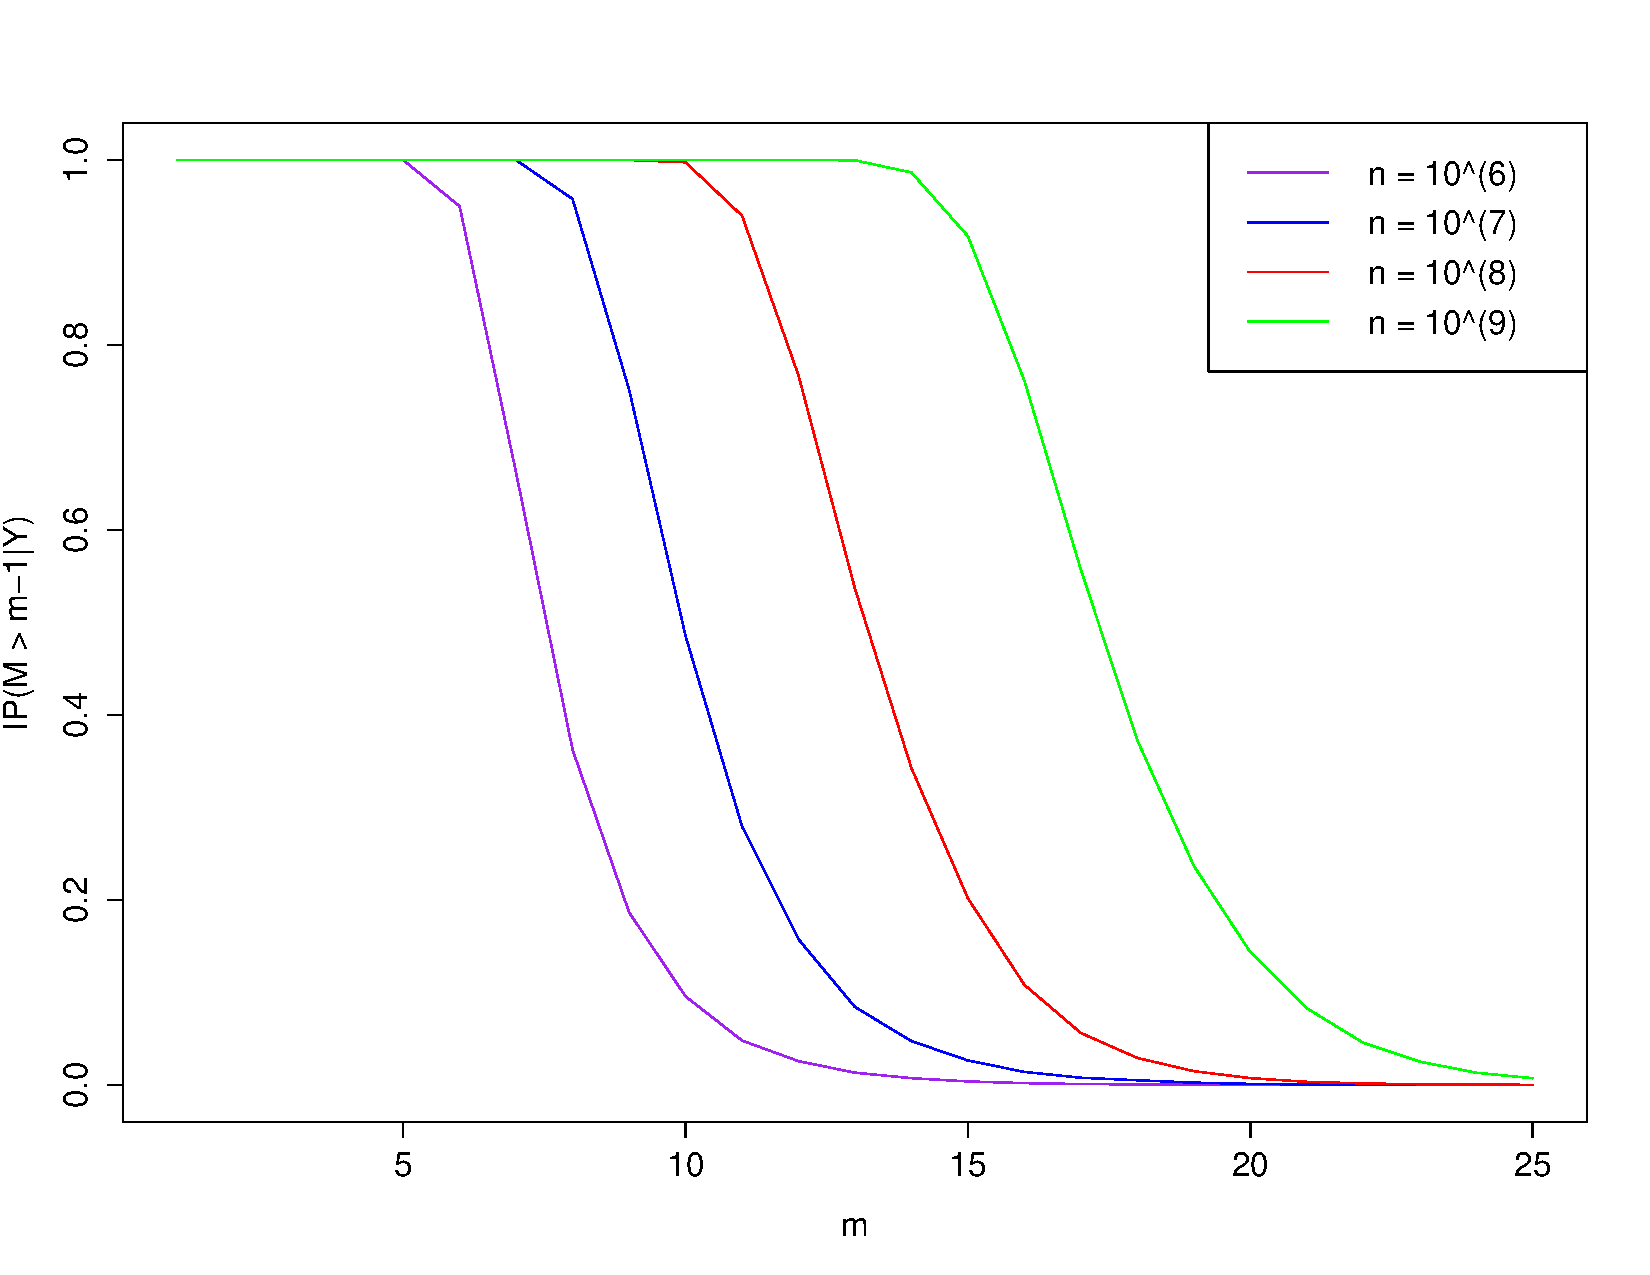
\includegraphics[width=.8\linewidth]{M.pdf}
\caption{Posterior survival function of $M$ for different values of $n$}\label{M}
\end{figure}
\end{frame}
%
%\begin{frame}{Explicit formulation}{Iterated posterior}
%We then fix the distribution of $M^{1}$: $\forall m \in \llbracket 1, G_{n} \rrbracket, $
%%\[\mathbb{P}_{M}(M = m) := \frac{\exp\left(-3 \cdot \eta \cdot \frac{m}{2} \right) \cdot \prod\limits_{j = 1}^{m} \left(1 + n \cdot \eta \cdot \lambda_{j}^{2}\right)^{2}}{\sum\limits_{k =1}^{G_{n}} \exp\left(-3 \cdot \eta \cdot \frac{k}{2} \right) \cdot \prod\limits_{j = 1}^{k} \left(1 + n \cdot \eta \cdot \lambda_{j}^{2}\right)^{2}}.\]
%\[\mathbb{P}_{M^{1}}(M = m) \propto \exp\left(-3 \cdot \eta \cdot \frac{m}{2} \right) \cdot \prod\limits_{j = 1}^{m} \left(1 + n \cdot \eta \cdot \lambda_{j}^{2}\right)^{2}.\]
%%\begin{columns} % Subdivide the first main column
%%\begin{column}{.5\textwidth} % The first subdivided column within the first main column
%Which gives the family of posterior distributions:
%\textcolor{red!90!black}{\[\mathbb{P}_{M^{\eta} \vert Y^{\eta}}^{n}(m) \propto \exp\!\!\left[- \frac{\eta}{2} \left( 3 m - \sum\limits_{j = 1}^{m} \frac{\eta\left(Y_{j} \cdot n \cdot \lambda_{j}^{2}\right)^{2}}{1 + \eta \cdot n \cdot \lambda_{j}^{2}} \right)\right].\]}
%\end{frame}

\section{Self-informative carrier/limit}
\begin{frame}{Self-informative carrier/limit}
\begin{block}{Proposition : Self informative limit \textbf{J \& L [2016]}}
As $\eta$ tends to $\infty$, the posterior mean $\widehat{\theta}^{\left(\eta\right)}$ converges almost surely towards the projection estimator given by the model selection $\widetilde{\theta}^{\widehat{m}}.$
\end{block}

\begin{block}{Proposition : Self informative Bayes carrier \textbf{J \& L [2016]}}
As $\eta$ tends to $\infty$, the posterior distribution $\mathbb{P}_{\boldsymbol{\theta}^{\eta}\vert Y^{\eta}}^{n}$ converges towards the degenerated distribution on the projection estimator given by the model selection $\delta_{\widetilde{\theta}^{\widehat{m}}}.$
\end{block}

Hence, $\eta$ introduces a form of continuum between the Bayes method and frequentist estimation.
%Consider the limit of the family of posteriors as $\eta$ tends to infinite:
%\[\textcolor{red!90!black}{\lim_{\eta \rightarrow \infty} \mathbb{P}_{\boldsymbol{\theta}^{\eta} \vert M^{\eta} = m, Y^{\eta}}^{n} = \delta_{\widetilde{\theta}^{m}}},\]
%where $\widetilde{\theta}^{m}$ is the projection estimator on the first $m$ dimensions.
%
%The distribution of $M$ tends to a point mass:
%\[\textcolor{red!90!black}{\lim_{\eta \rightarrow \infty} \mathbb{P}_{M^{\eta}\vert Y^{\eta}}^{n} = \delta_{\widehat{m}}},\]
%where $\widehat{m}$ is the choice given by the frequentist model selection presented earlier.
%
%\medskip
%
%The \textcolor{red}{self-informative limit} is equal to the model selection estimator, $\widehat{\theta}$, presented above.
\end{frame}

%\begin{frame}{Self-informative carrier/limit}{Graphic representation}
%\begin{figure}
%\centering
% 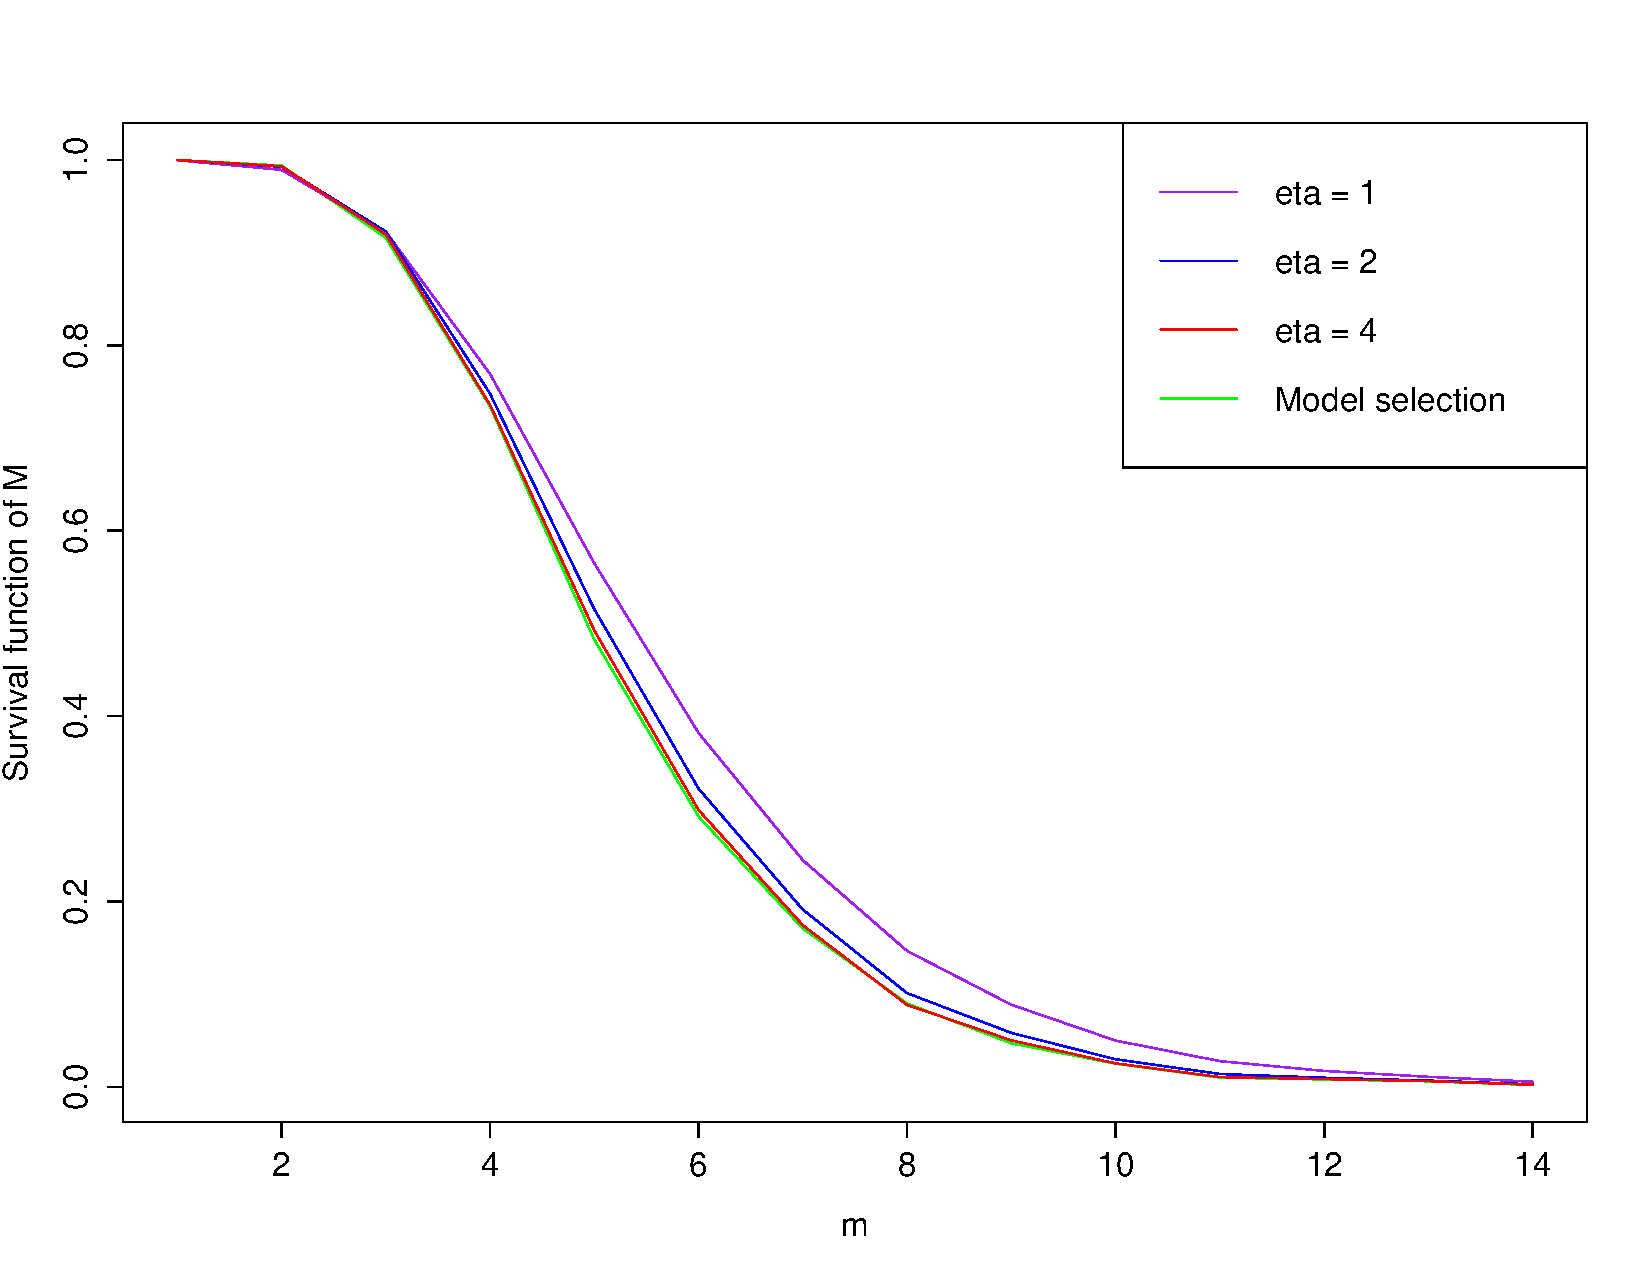
\includegraphics[width=.8\linewidth]{iteration.pdf}
%\caption{Survival function of $M^{\eta}\vert Y^{\eta}$ for different values of $\eta$}\label{iteration}
%\end{figure}
%\end{frame}

\section{Optimality}

\subsection{Frequentist case}
\begin{frame}{Formulation of optimality}{Frequentist case}
\begin{columns}
\begin{column}[T]{.4\textwidth}%
\hspace*{8ex}\includegraphics<1-2>[scale=.8]{inv-gssm-minimax.1}%
\includegraphics<3>[scale=.8]{inv-gssm-minimax.2}% lower
\includegraphics<4>[scale=.8]{inv-gssm-minimax.3}%
\includegraphics<5>[scale=.8]{inv-gssm-minimax.4}%
\includegraphics<6>[scale=.8]{inv-gssm-minimax.5}% upper + lower
\includegraphics<7>[scale=.8]{inv-gssm-minimax.6}%
\includegraphics<8->[scale=.8]{inv-gssm-minimax.7}%
\begin{textblock}{6}(2,14.5) \only<1->{Parameter of interest}\end{textblock} 
\end{column}\begin{column}[T]{.7\textwidth}%
\begin{itemize}
\item<2->
For each frequentist estimator, consider the {\textcolor{red}{maximal risk}} 
over a  class $\Theta^{\circ}$  of parameters
  \begin{equation*}
\sup\limits_{\theta^{\circ} \in \Theta^{\circ}} \mathbb{E}_{\theta^{\circ}}^{n} \left[d\left(\widetilde{\theta}, \theta^{\circ}\right)^{2}\right].
\end{equation*}
 \item<3->  Goal: \textcolor{red!90!black}{derive a lower bound} for this risk
\begin{equation*}
\inf\limits_{\widetilde{\theta}}\sup\limits_{\theta^{\circ} \in \Theta^{\circ}} \mathbb{E}_{\theta^{\circ}}^{n}\left[d\left(\widetilde{\theta}, \theta^{\circ}\right)^{2}\right] \geq \mathcal{R}_{n}^{\star}\left(\Theta^{\circ}\right).
\end{equation*}
\item<8-> Finding $\widehat{\theta}$ such that
  \begin{equation*}
\sup\limits_{\theta^{\circ}\in \Theta^{\circ}} \mathbb{E}_{\theta^{\circ}}^{n}\left[d\left(\widehat{\theta}, \theta^{\circ}\right)^{2}\right] \leq K^{\star} \cdot \mathcal{R}_{n}^{\star}\left(\Theta^{\circ}\right),
\end{equation*}
it is then \textcolor{red!90!black}{minimax rate optimal} and \textcolor{red!90!black}{adaptive} if $\widehat{\theta}$ does not depend on $\Theta^{\circ}$.
\end{itemize}
\end{column}
\end{columns}
\end{frame}

\subsection{Pragmatic Bayesian case}
\begin{frame}{Formulation of optimality}{Pragmatic Bayesian paradigm}
How to transfer this in a Bayesian point of view ?

\bigskip

Taking a "pragmatic Bayesian" point of view :

\bigskip

\begin{itemize}
\setlength\itemsep{3em}
\item $\theta^{\circ}$ the \textcolor{red!90!black}{true parameter}.
\item Is $\mathbb{P}_{\boldsymbol{\theta}\vert Y}^{n}$ \textcolor{red!90!black}{shrinking} around $\theta^{\circ}$ as $n$ tends to $\infty$ ?
\item How fast ?

\end{itemize}

\end{frame}


\begin{frame}{Formulation of optimality}{Pragmatic Bayesian formulation of optimality}
\begin{columns}
\begin{column}[T]{.4\textwidth}%
\hspace*{4ex}\includegraphics<1>[scale=.8]{reg.31}%
\includegraphics<2>[scale=.8]{reg.32}%
\includegraphics<3>[scale=.8]{reg.33}%
\includegraphics<4>[scale=.8]{reg.34}%
\includegraphics<5>[scale=.8]{reg.35}%
\includegraphics<6>[scale=.8]{reg.36}%
\includegraphics<7>[scale=.8]{reg.37}%
\includegraphics<8->[scale=.8]{reg.38}%
\end{column}\begin{column}[T]{.7\textwidth}%

\begin{itemize}

\item<1-> \textcolor{red!90!black}{Concentration rate} $(\phi_{n})_{n \in \mathbb{N}}$
\[\exists c \in \mathbb{R}_{+}, \quad \lim_{n \rightarrow \infty} \mathbb{E}_{\theta^{\circ}}^{n}\left[ \mathbb{P}_{\boldsymbol{\theta}\vert Y}^{n} \left(d\left(\boldsymbol{\theta}, \theta^{\circ} \right)^{2} \geq c \, \phi_{n} \right) \right] = 0. \]

\item<5-> \textcolor{red!90!black}{Exact concentration rate} $(\phi_{n})_{n \in \mathbb{N}}$ if in addition

\[ \lim_{n \rightarrow \infty} \mathbb{E}_{\theta^{\circ}}^{n}\left[ \mathbb{P}_{\boldsymbol{\theta}\vert Y}^{n} \left(d\left(\boldsymbol{\theta}, \theta^{\circ} \right)^{2} \leq c^{-1} \, \phi_{n} \right) \right] = 0. \]

\end{itemize}
\end{column}
\end{columns}

\end{frame}

\begin{frame}{Formulation of optimality}{Pragmatic Bayesian formulation of minimax optimality}
\begin{itemize}
\item Uniform concentration rate $(\phi_{n})_{n \in \mathbb{N}}$ over a subset on $\Theta^{\circ} \subset \Theta$
\[  \lim_{n \rightarrow \infty} \sup_{\theta^{\circ} \in \Theta^{\circ}} \mathbb{E}_{\theta^{\circ}}^{n}\left[ \mathbb{P}_{\boldsymbol{\theta}\vert Y}^{n} \left(d\left( \boldsymbol{\theta}, \theta^{\circ} \right)^{2} \geq c \, \phi_{n} \right) \right] = 0.\]

\item Exact uniform concentration rate $(\phi_{n})_{n \in \mathbb{N}}$ if in addition
\[ \lim_{n \rightarrow \infty} \sup_{\theta^{\circ} \in \Theta^{\circ}} \mathbb{E}_{\theta^{\circ}}^{n}\left[ \mathbb{P}_{\boldsymbol{\theta}\vert Y}^{n} \left(d\left( \boldsymbol{\theta}, \theta^{\circ} \right)^{2} \leq c^{-1} \, \phi_{n} \right) \right] = 0. \]

\end{itemize}
\end{frame}

\subsection{Definitions}
\begin{frame}{Existing optimality results}{Definitions}

We here note :
\begin{itemize}
\item $\Phi_{n}^{\circ} = \Phi_{n}^{\circ}\left(\theta^{\circ}\right)$ the optimal convergence rate for the family of projection estimators for each $\theta^{\circ}$;
\item $\Phi_{n}^{\star} = \Phi_{n}^{\star}\left(\Theta^{\circ}\right)$ the minimax optimal convergence rate over some Sobolev ellipsoid $\Theta^{\circ}$.
\end{itemize}
Those objects have analytical formulation (see for example \textbf{\citet{JJMS}}).

\end{frame}

%\subsection{Assumptions}
%\begin{frame}{Existing optimality results}{Assumptions}
%Define the following assumptions:
%\begin{alignat*}{2}
%&\left(\mathbb{H}_{\lambda}\right) &&: \exists a \in \mathbb{R}_{+}, c \geq 1 : \quad \forall j \in \mathbb{N}, \quad \left(\frac{1}{c} j^{-a} \leq \lambda_{j} \leq c j^{-a}\right)\\
%&\left(\mathbb{H}_{1}\right) &&: 0 <\inf\limits_{n \in \mathbb{N}} \left\{\frac{\left[\textgoth{b}_{m_{n}^{\circ}}\wedge n^{-1} m_{n}^{\circ} \overline{\Lambda}_{m_{n}^{\circ}}\right]}{\left[\textgoth{b}_{m_{n}^{\circ}}\vee n^{-1} m_{n}^{\circ} \overline{\Lambda}_{m_{n}^{\circ}}\right]}\right\} \leq 1\\
%&\left(\mathbb{H}_{2}\right) &&: 0 <\inf\limits_{n \in \mathbb{N}} \left\{\frac{\left[\textgoth{a}_{m_{n}^{\star}}\wedge n^{-1} m_{n}^{\star} \overline{\Lambda}_{m_{n}^{\star}}\right]}{\left[\textgoth{a}_{m_{n}^{\star}}\vee n^{-1} m_{n}^{\star} \overline{\Lambda}_{m_{n}^{\star}}\right]}\right\} \leq 1\\
%\end{alignat*}
%\end{frame}

%\subsection{Optimality of the Bayes estimate}
%\begin{frame}{Existing optimality results}{Optimality of the Bayes estimate}
%In \citet{JJASRS}, it is shown that the estimator $\widehat{\theta}^{\left(1\right)}$ \textcolor{red!90!black}{converges with,}
%	\begin{itemize}
%		\item \textcolor{red!90!black}{oracle optimal rate} for the quadratic risk which means, $\forall \theta^{\circ} \in \Theta^{\circ}, \exists C^{\circ} \in \left[ 1, \infty \right[ : \forall n \in \mathbb{N}:$
%		\begin{alignat*}{2}
%&\inf\limits_{m \in \mathbb{N}} \, && \mathbb{E}_{\theta^{\circ}}^{n}\left[\left\Vert \widetilde{\theta}^{m} - \theta^{\circ} \right\Vert^{2}\right] \geq \Phi_{n}^{\circ},\\
%& && \mathbb{E}_{\theta^{\circ}}^{n}\left[\left\Vert \widehat{\theta}^{\left(1\right)} - \theta^{\circ} \right\Vert^{2}\right] \leq C^{\circ} \Phi_{n}^{\circ};
%		\end{alignat*}
%		\item \textcolor{red!90!black}{minimax optimal rate} for the maximal risk over $\Theta^{\circ}$, that is to say, $\exists C^{\star} \in \left[ 1, \infty \right[ : \forall n \in \mathbb{N}:$
%\begin{alignat*}{2}
%& \inf\limits_{\widetilde{\theta}} &&\sup\limits_{\theta^{\circ} \in \Theta^{\circ}} \mathbb{E}_{\theta^{\circ}}^{n}\left[\left\Vert \widetilde{\theta} - \theta^{\circ} \right\Vert^{2}\right] \geq \Phi_{n}^{\star},\\
%& && \sup\limits_{\theta^{\circ} \in \Theta^{\circ}} \mathbb{E}_{\theta^{\circ}}^{n}\left[\left\Vert \widehat{\theta}^{\left(1\right)} - \theta^{\circ} \right\Vert^{2}\right] \leq C^{\star} \Phi_{n}^{\star},
%\end{alignat*}
%where $\inf\limits_{\widetilde{\theta}}$ is taken over all possible estimators of $\theta^{\circ}$.
%	\end{itemize}
%
%\end{frame}
%
%\subsection{Optimality of the posterior distribution}
%\begin{frame}{Existing optimality results}{Optimality of the posterior distribution}
%It is also shown that the posterior distribution \textcolor{red!90!black}{concentrates with,}
%	\begin{itemize}
%		\item \textcolor{red!90!black}{oracle optimal rate} for the quadratic loss which means, $\forall \theta^{\circ} \in \Theta^{\circ}, \exists K^{\circ} \in \left[ 1, \infty \right[ :$
%\[\lim\limits_{n \rightarrow \infty} \mathbb{E}_{\theta^{\circ}}^{n}\left[\mathbb{P}_{\boldsymbol{\theta}^{1}\vert Y^{1}}^{n}\left(\left\Vert \boldsymbol{\theta} - \theta^{\circ} \right\Vert^{2} \leq K^{\circ} \Phi_{n}^{\circ}\right)\right] = 1;\]
%		\item \textcolor{red!90!black}{minimax optimal rate} $\Theta^{\circ}$, that is to say, for any unbounded sequence $K_{n} \in \mathbb{R}^{\mathbb{N}} :$
%\[\lim\limits_{n \rightarrow \infty} \sup\limits_{\theta^{\circ} \in \Theta^{\circ}}  \mathbb{E}_{\theta^{\circ}}^{n}\left[\mathbb{P}_{\boldsymbol{\theta}^{1}\vert Y^{1}}^{n}\left(\left\Vert \boldsymbol{\theta} - \theta^{\circ} \right\Vert^{2} \leq K_{n} \Phi_{n}^{\star}\right)\right] = 1.\]
%	\end{itemize}
%\end{frame}

%\subsection{Optimality of the hyper-parameter}
%\begin{frame}{Optimality of the iterated version}{Optimality of the hyper-parameter - oracle optimal choice}
%A key argument for optimality is that, for any $\eta$, the posterior distribution of the hyper-parameter $M^{\eta}$ concentrates around the optimal thresholds $m_{n}^{\circ}$ and $m_{n}^{\star}$ as $n$ tends to infinity.
%\end{frame}


%\section{Optimality of the iterated version}
%\subsection{Optimality of the hyper-parameter}
%\begin{frame}{Optimality of the iterated version}{Optimality of the hyper-parameter - oracle optimal choice}
%For any $\eta$ in $\overline{\mathbb{N}},$ we have the following results:
%
%\medskip
%
%Under assumptions $\left(\mathbb{H}_{1}\right)$ and $\left(\mathbb{H}_{\lambda}\right)$, define
%\begin{alignat*}{2}
%&G_{n}^{-} &&:= \min\left\{m \in \llbracket 1, m_{n}^{\circ} \rrbracket : \textgoth{b}_{m} \leq 9 L \Phi_{n}^{\circ}\right\},\\
%&G_{n}^{+} &&:= \max \left\{m \in \llbracket m_{n}^{\circ}, G_{n} \rrbracket : \left( m - m_{n}^{\circ} \right) n^{-1} \leq 3 \Lambda_{m_{n}^{\circ}}^{-1} \Phi_{n}^{\circ}\right\},
%\end{alignat*}
%and we then have the following concentration for $M$,
%\begin{alignat*}{4}
%&\mathbb{P}_{\theta^{\circ}}&&\left[M^{\eta} > G_{n}^{+}\right] &&\leq&& \exp\left[- \frac{5 m_{n}^{\circ}}{9 L} + \log \left(G_{n}\right)\right],\\
%&\mathbb{P}_{\theta^{\circ}}&&\left[M^{\eta} < G_{n}^{-}\right] &&\leq&& \exp\left[- \frac{7 m_{n}^{\circ}}{9} + \log \left(G_{n}\right)\right],
%\end{alignat*}
%\textcolor{red!90!black}{this means that $M^{\eta}$ tends to select an oracle optimal threshold}.
%\end{frame}
%
%
%\begin{frame}{Optimality of the iterated version}{Optimality of the hyper-parameter- minimax optimal choice}
%For any $\eta$ in $\overline{\mathbb{N}},$ we have the following results:
%
%under $\left(\mathbb{H}_{2}\right)$ and $\left(\mathbb{H}_{\lambda}\right)$, we define
%\begin{alignat*}{2}
%&G_{n}^{\star-} &&:= \min\left\{m \in \llbracket 1, m_{n}^{\star} \rrbracket : \quad \textgoth{b}_{m} \leq 9 \left(1 \vee L^{\circ}\right) L \Phi_{n}^{\star}\right\},\\
%&G_{n}^{\star+} &&:= \max \left\{m \in \llbracket m_{n}^{\star}, G_{n} \rrbracket : \left( m - m_{n}^{\star} \right) n^{-1} \leq 3 \Lambda_{m_{n}^{\star}}^{-1} \left(1 \vee L^{\circ}\right) \Phi_{n}^{\star}\right\},
%\end{alignat*}
%and the following concentration stands,
%\begin{alignat*}{4}
%&\mathbb{P}_{\theta^{\circ}}&&\left[M^{\eta} > G_{n}^{\star+}\right] &&\leq &&\exp\left[- \frac{5 \left(1 \vee L^{\circ}\right) m_{n}^{\star}}{9 L} + \log \left(G_{n}\right)\right],\\
%&\mathbb{P}_{\theta^{\circ}}&&\left[M^{\eta} < G_{n}^{\star-}\right] &&\leq &&\exp\left[- \frac{7 \left(1 \vee L^{\circ}\right) m_{n}^{\star}}{9} + \log \left(G_{n}\right)\right],
%\end{alignat*}
%\textcolor{red!90!black}{which means that $M^{\eta}$ tends to select a minimax optimal threshold}.
%\end{frame}


\subsection{Optimality of the iterated Bayes estimate}
\begin{frame}{Optimality of the iterated version}{Optimality of the iterated Bayes estimate}
\begin{block}<1->{Theorem : oracle optimality \textbf{J \& L [2016]}}
For all $\theta^{\circ}$ in $\Theta^{\circ}$ and all fixed $\eta$ in $\mathbb{N}^{\star} \cup \infty$, there exist $C^{\circ}$ such that
	\[\forall n, \in \mathbb{N}^{\star}, \quad \mathbb{E}_{\theta^{\circ}}^{n}\left[\Vert \widehat{\theta}^{\left(\eta\right)} - \theta^{\circ} \Vert^{2}\right] \leq C^{\circ} \Phi_{n}^{\circ};\]
\end{block}
\begin{block}<2->{Theorem : minimax optimality \textbf{J \& L [2016]}}
For all fixed $\eta$ in $\mathbb{N}^{\star} \cup \infty$, there exist $C^{\star}$ such that
	\[\forall n \in \mathbb{N}^{\star}, \quad \sup\limits_{\theta^{\circ}\in \Theta^{\circ}}\mathbb{E}_{\theta^{\circ}}^{n}\left[\Vert \widehat{\theta}^{\left(\eta\right)} - \theta^{\circ} \Vert^{2}\right] \leq C^{\star} \Phi_{n}^{\star}.\]
\end{block}
The case $\eta = 1$ was already studied in \textbf{\citet{JJASRS}}.
\end{frame}

\subsection{Optimality of the iterated posterior}
\begin{frame}{Optimality of the iterated version}{Optimality of the iterated posterior}

\begin{block}{Theorem \textbf{J \& L [2016]}}
First, we underline that $\Phi_{n}^{\circ}$ and $\Phi_{n}^{\star}$ can be considered as upper bounds for the family of sieve priors:
\begin{itemize}
\item $\lim\limits_{n \rightarrow \infty} \inf\limits_{\mathbb{Q}_{\boldsymbol{\theta}}}\, \mathbb{E}_{\theta^{\circ}}^{n}\left[\mathbb{Q}_{\boldsymbol{\theta} \vert Y}^{n}\left(\left\Vert \boldsymbol{\theta} - \theta^{\circ} \right\Vert^{2} \geq \Phi_{n}^{\circ}\right)\right] = 1$,
\item $\lim\limits_{n \rightarrow \infty} \inf\limits_{\mathbb{Q}_{\boldsymbol{\theta}}}\sup\limits_{\theta^{\circ} \in \Theta^{\circ}}\, \mathbb{E}_{\theta^{\circ}}^{n}\left[\mathbb{Q}_{\boldsymbol{\theta} \vert Y}^{n}\left(\left\Vert \boldsymbol{\theta} - \theta^{\circ} \right\Vert^{2} \geq \Phi_{n}^{\star}\right)\right] = 1$,
\end{itemize}
where $\inf_{\mathbb{Q}_{\boldsymbol{\theta}}}$ is taken over the family of sieve priors.
\end{block}
The first expression gives a purely Bayesian formulation of oracle optimality.

Could the second expression be a first step towards a purely Bayesian formulation of minimax optimality ?
\end{frame}

\begin{frame}{Optimality of the iterated version}{Optimality of the iterated posterior}
\begin{block}<1->{Theorem : oracle concentration \textbf{J \& L [2016]}}
For all $\theta^{\circ}$ in $\Theta^{\circ}$ and all fixed $\eta$ in $\mathbb{N}^{\star} \cup \infty$, there exist $K^{\circ}$ such that
	\[\lim\limits_{n \rightarrow \infty} \mathbb{E}_{\theta^{\circ}}^{n}\left[\mathbb{P}_{\boldsymbol{\theta}^{\eta}, M^{\eta} \vert Y^{\eta}}^{n}\left(\left(K^{\circ}\right)^{-1} \Phi_{n}^{\circ} \leq \Vert \boldsymbol{\theta} - \theta^{\circ} \Vert^{2} \leq K^{\circ} \Phi_{n}^{\circ} \right)\right] = 1;\]
\end{block}
\begin{block}<2->{Theorem : minimax concentration \textbf{J \& L [2016]}}
for all fixed $\eta$ in $\mathbb{N}^{\star} \cup \infty$, and any unbounded sequence $K_{n}$, we have
	\[\lim\limits_{n \rightarrow \infty} \sup\limits_{\theta^{\circ} \in \Theta^{\circ}} \mathbb{E}_{\theta^{\circ}}^{n}\left[\mathbb{P}_{\boldsymbol{\theta}^{\eta}, M^{\eta} \vert Y^{\eta}}^{n}\left(\Vert \boldsymbol{\theta} - \theta^{\circ} \Vert^{2} \leq K_{n} \Phi_{n}^{\star} \right)\right] = 1.\]
	\end{block}

For $\eta \rightarrow \infty$, this gives convergence in probability.
%\[\lim\limits_{\eta \rightarrow \infty}\mathbb{E}_{\theta^{\circ}}^{n}\left[\mathbb{P}_{\boldsymbol{\theta}^{\eta}, M^{\eta} \vert Y^{\eta}}^{n}\left(\Vert \boldsymbol{\theta} - \theta^{\circ} \Vert^{2} \leq K_{n} \Phi_{n} \right)\right] = \mathbb{P}_{\theta^{\circ}}^{n}\left[\Vert \widehat{\theta} - \theta^{\circ} \Vert^{2} \leq K_{n} \Phi_{n}\right].\]

The case $\eta = 1$ was already studied in \textbf{\citet{JJASRS}}.
\end{frame}

\begin{frame}{Simulations}{Evolution of MSE}
\begin{figure}
\centering
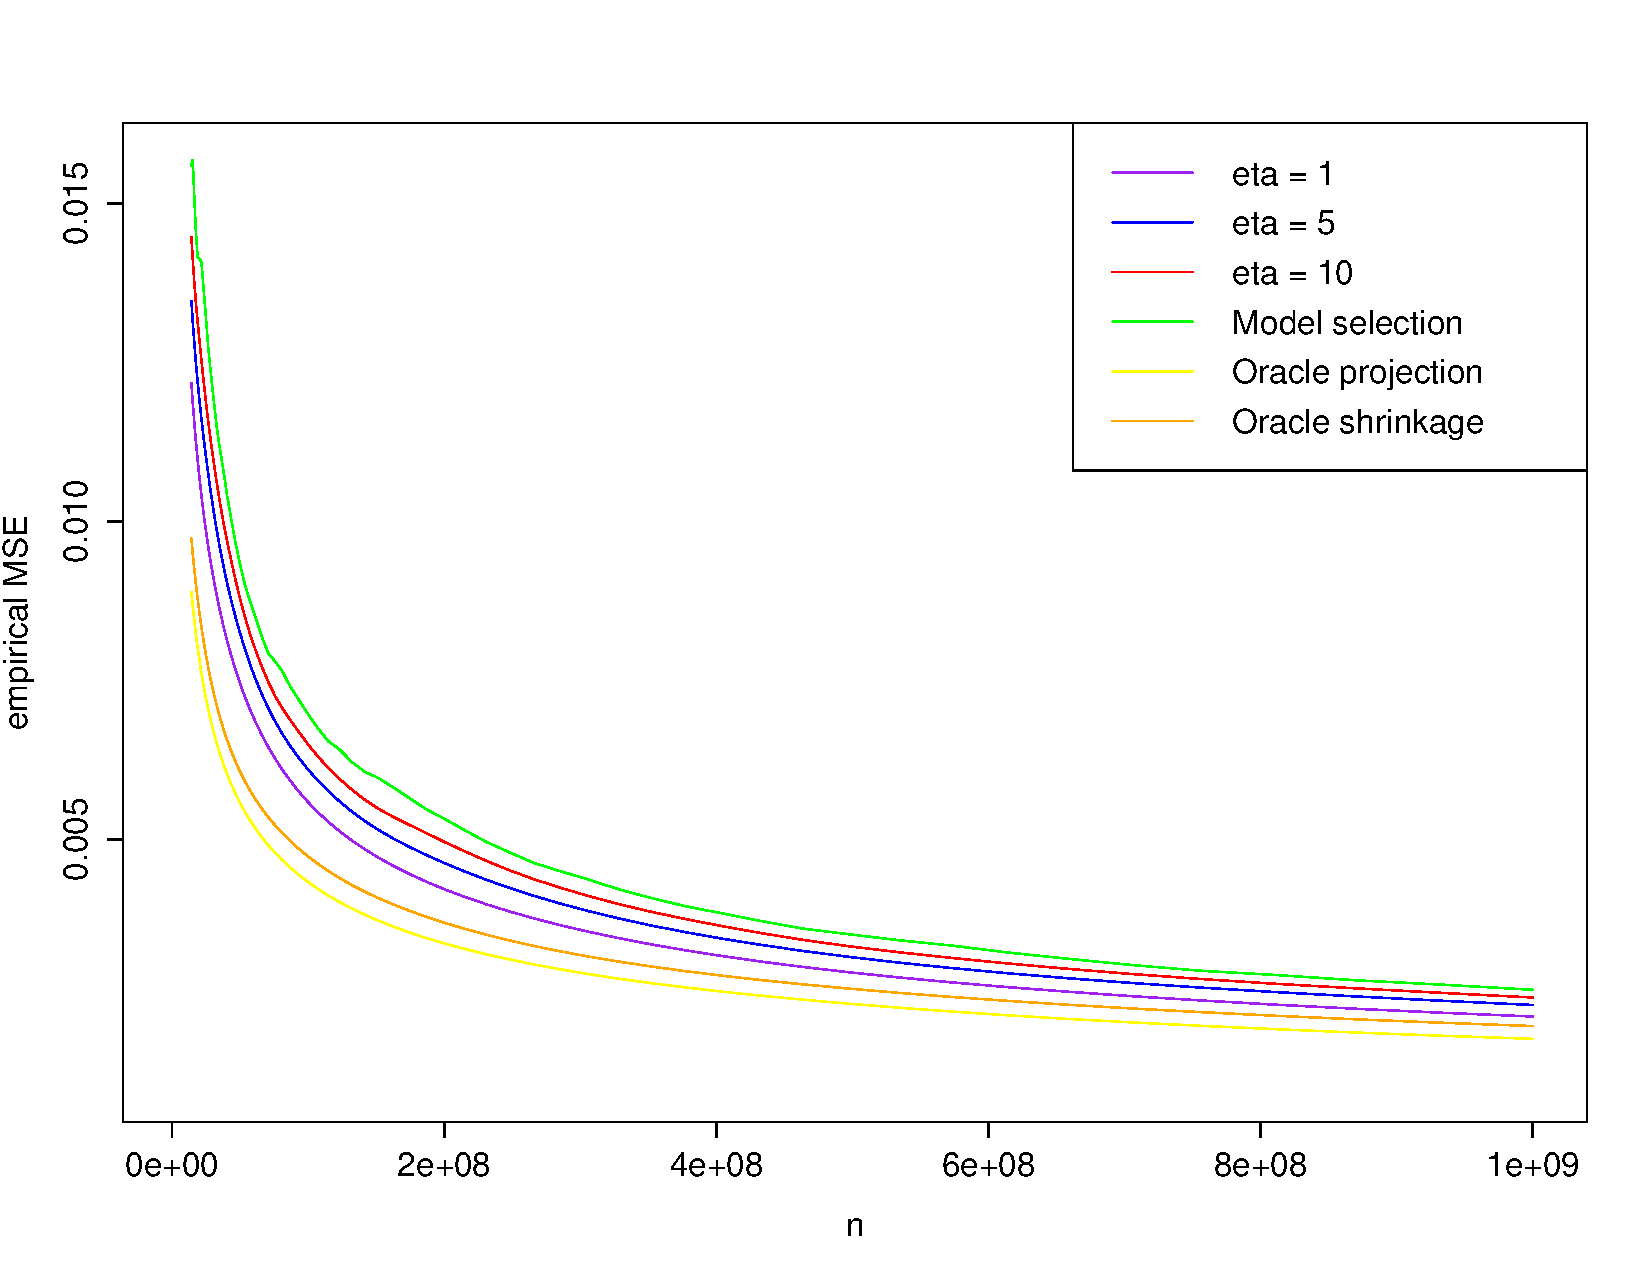
\includegraphics[width=.9\linewidth]{EQM1.pdf}
\end{figure}
\end{frame}

\begin{frame}{Simulations}{Posterior distribution in direct case}
\begin{figure}
\centering
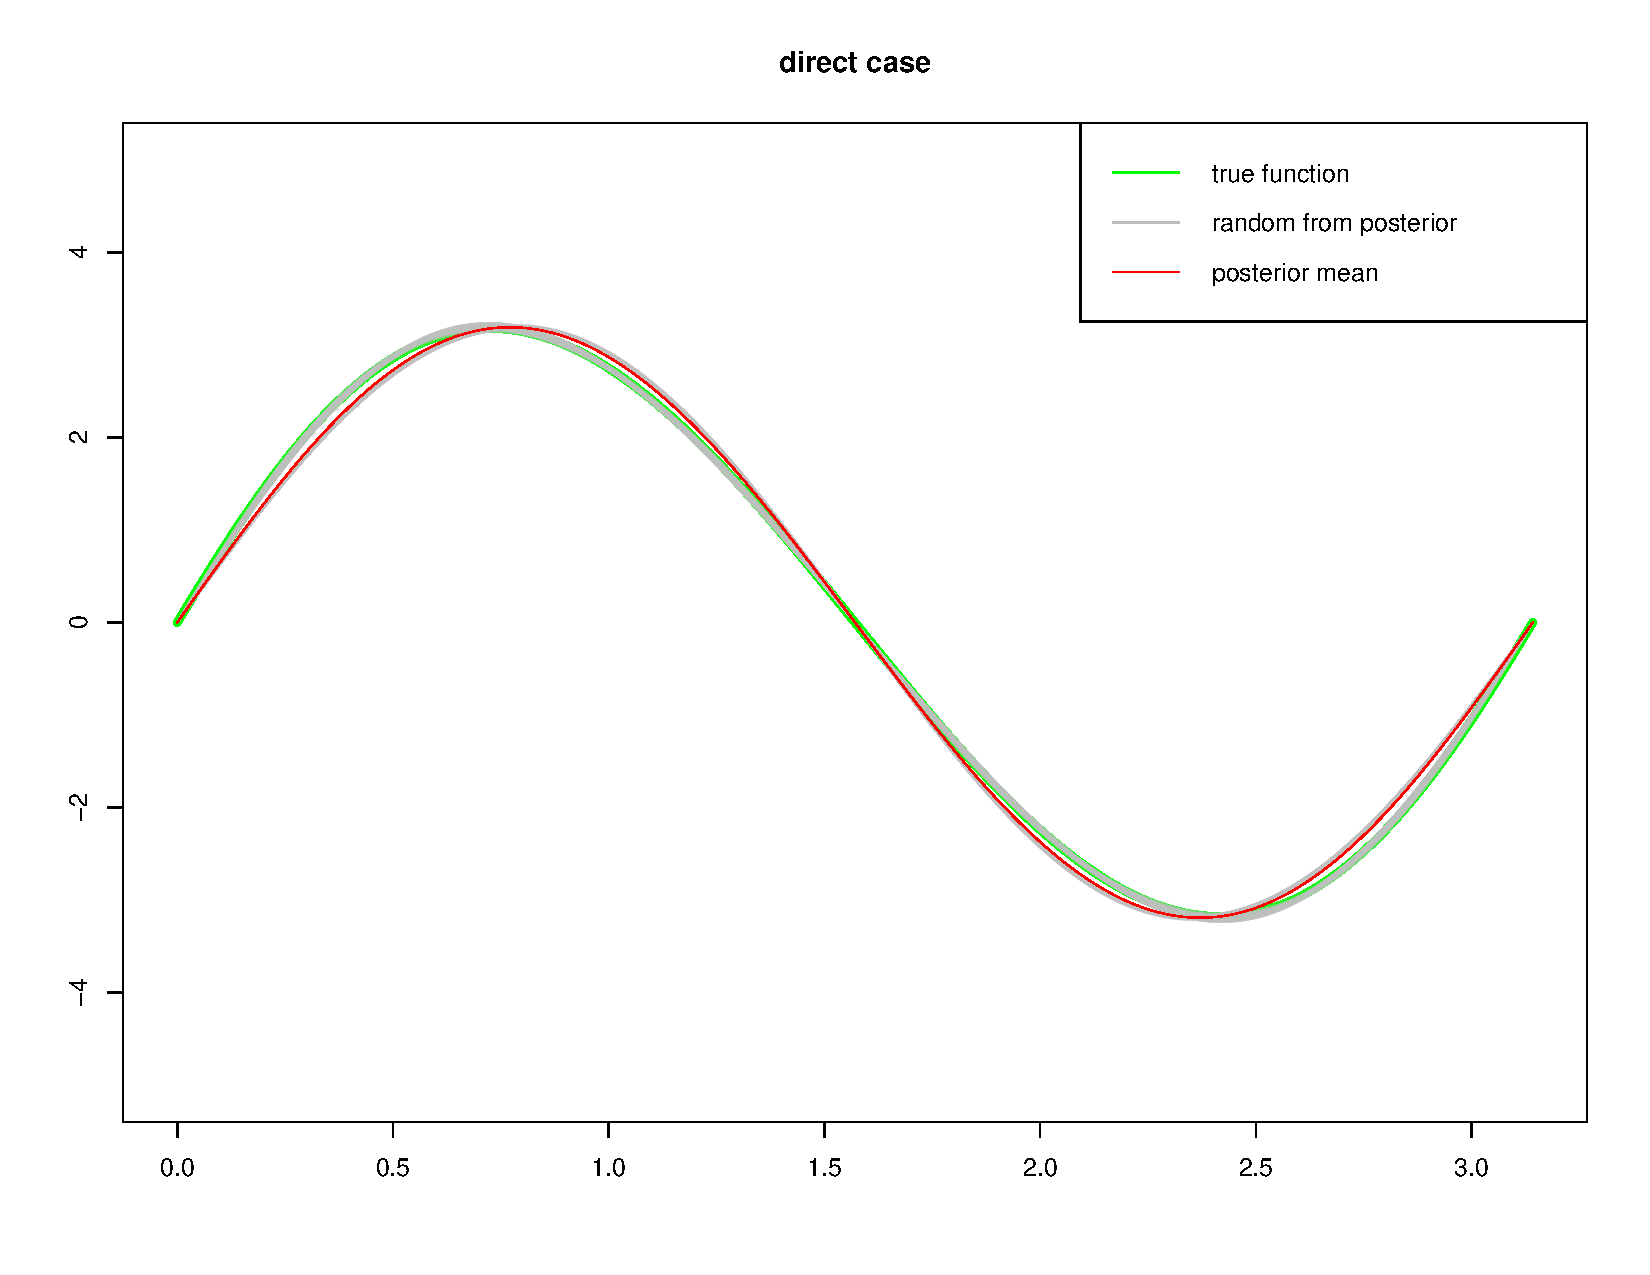
\includegraphics[width=.9\linewidth]{tirage-direct.pdf}
\end{figure}
\end{frame}

\begin{frame}{Simulations}{Posterior distribution in inverse case}
\begin{figure}
\centering
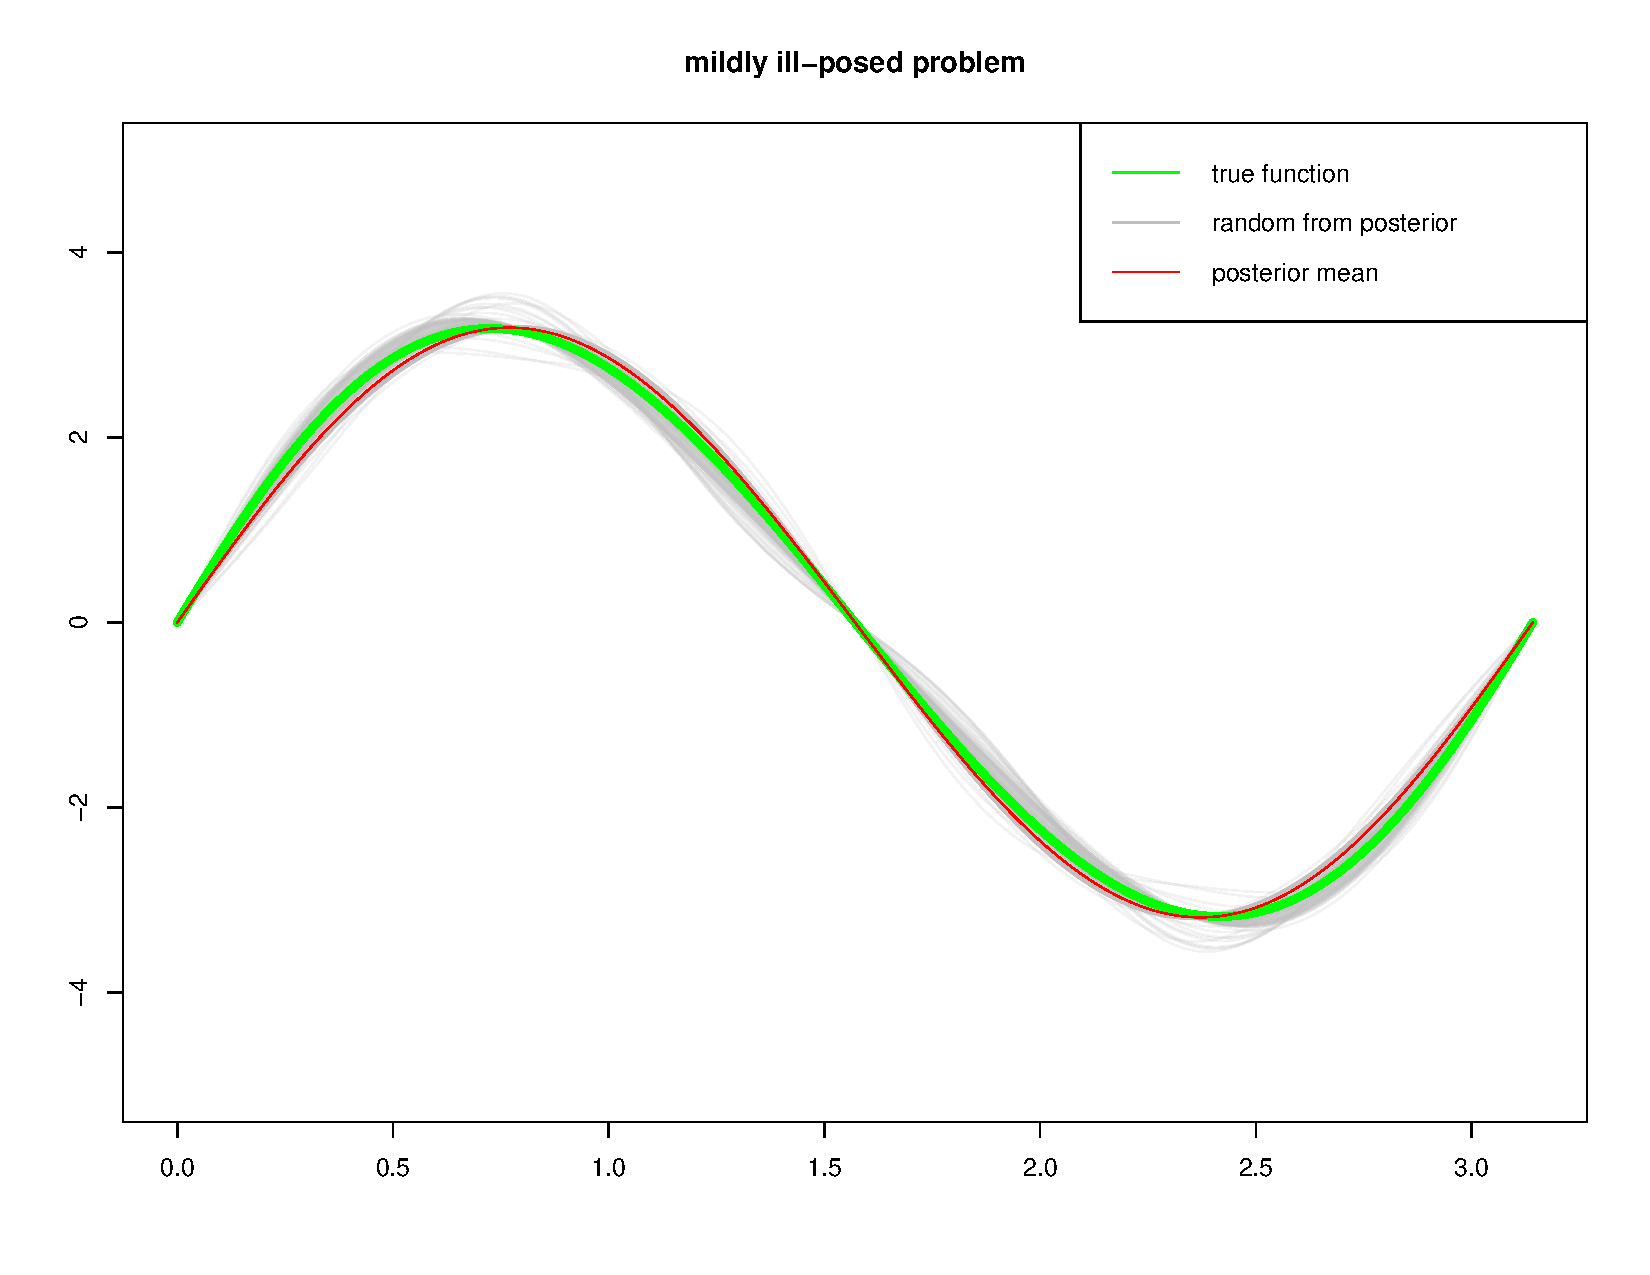
\includegraphics[width=.9\linewidth]{tirage-inverse.pdf}
\end{figure}
\end{frame}

\begin{frame}{Summary}
\begin{itemize}
\setlength\itemsep{2em}
\item Family of Bayesian methods indexed by an iteration parameter ;
\item frequentist "model selection" method  is a limit case ;
\item optimality of the estimators given by the posterior means ;
\item optimal concentration rate of the posterior distributions ;
\item first step towards a Bayesian formulation of minimax optimality ?
\end{itemize}
\end{frame}

\begin{frame}<beamer:0>
\bibliography{iGSSM}
\end{frame}
\bibliographystyle{plainnat}
\end{document}